\documentclass[cn]{homework}

\title{作业12}

\begin{document}
    \maketitle

    \problem[题2]
    直接绘制出\code{Tbill,r5,r10}的数据(\cref{fig:ts}),很明显它们是非平稳的。
    同时ADF检验(\cref{tab:ADF 3})也表明了同样的结论。
    \begin{figure}[h]
        \centering
        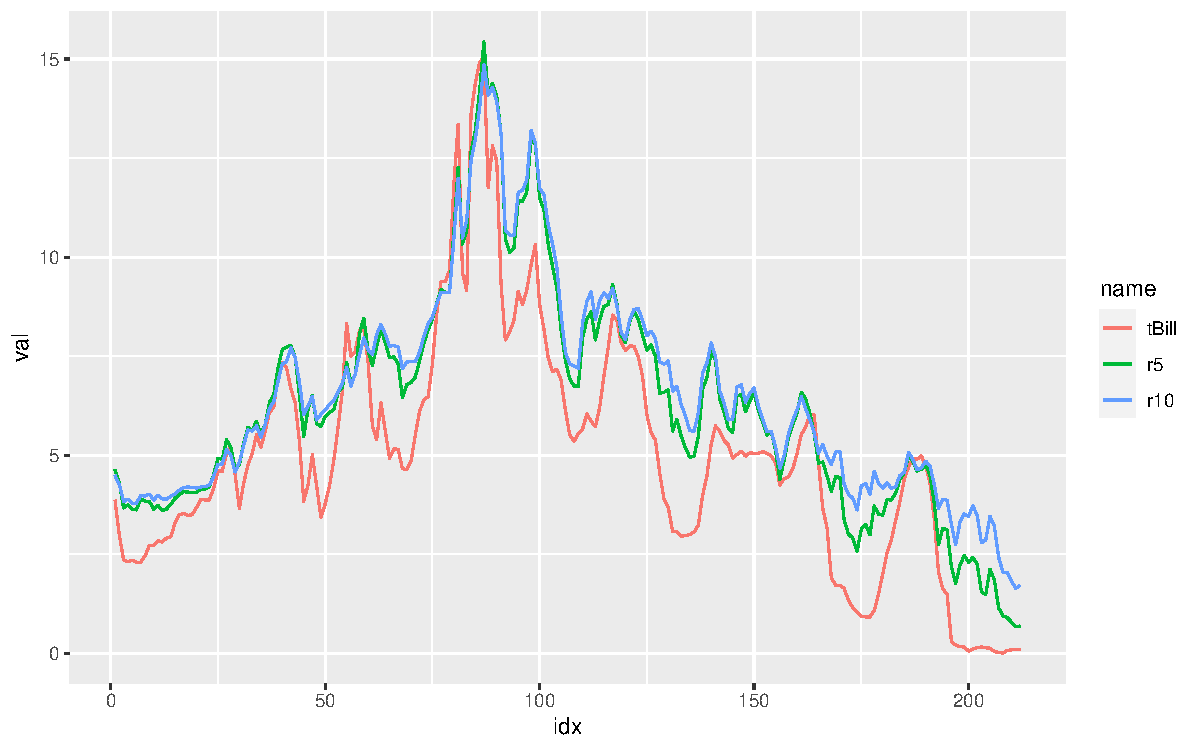
\includegraphics[width=\textwidth]{ts}
        \caption{时序图}
        \label{fig:ts}
    \end{figure}

    \begin{margintable}
        \centering
        \begin{tabular}{ccccc}
            \toprule
            滞后阶数 & Tbill & r5 & r10 \\
            \midrule
            1 & 0.532 & 0.749 & 0.766 \\
            2 & 0.298 & 0.571 & 0.588 \\
            3 & 0.505 & 0.682 & 0.641 \\
            4 & 0.209 & 0.525 & 0.540 \\
            5 & 0.314 & 0.575 & 0.580 \\
            \bottomrule
        \end{tabular}
        \caption{不同滞后阶数下ADF检验$p$值(带常数项)}
        \label{tab:ADF 3}
    \end{margintable}

    直接用\code{Tbill}对\code{r5,r10}回归可以得到
    回归表达式
    \[Tbill=0.3668+2.7430\cdot r5-1.9055\cdot r10\]
    其残差的图像上来看(\cref{fig:resid})大致是平稳的,
    同时做ADF检验,$p$值(如\cref{tab:ADF resid})均显著小于0.05,故认为是平稳的,
    由此可以得出存在协整关系的结论,同时协整向量由
    上面OLS估计式给出。

    \begin{marginfigure}
        \centering
        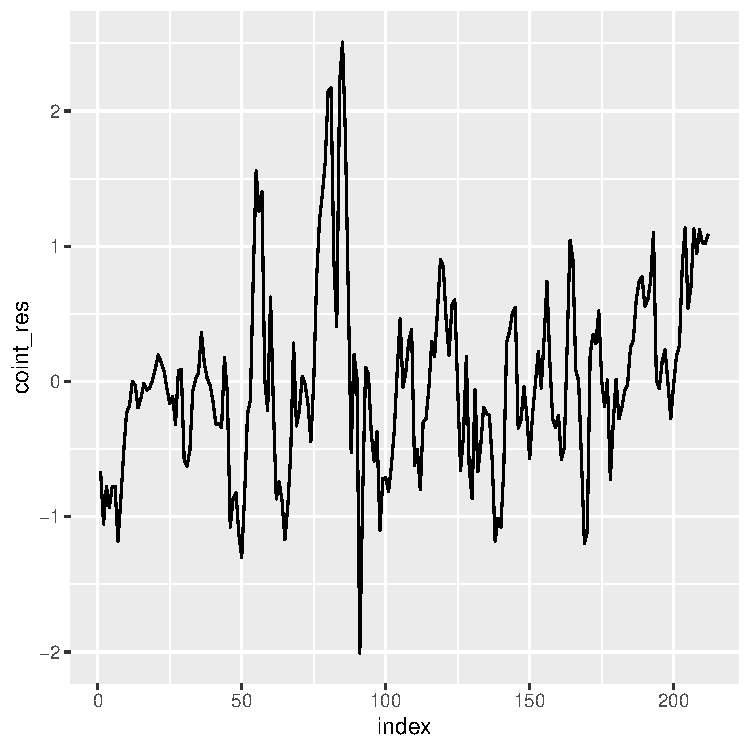
\includegraphics[width=\textwidth]{residual}
        \caption{残差图}
        \label{fig:resid}
    \end{marginfigure}

    \begin{margintable}
        \centering
        \begin{tabular}{cc}
            \toprule
            滞后阶数 & $p值$ \\
            \midrule
            1 & 0.01 \\ 
            2 & 0.01 \\ 
            3 & 0.01 \\ 
            4 & 0.01 \\ 
            5 & 0.01 \\ 
            \bottomrule
        \end{tabular}
        \caption{不同滞后阶数下ADF检验$p$值(带常数项)}
        \label{tab:ADF resid}
    \end{margintable}

    下面考虑建立ECM模型,直接对$\Delta Tbill,\Delta r5, \Delta r10,\hat u_t$
    进行无常数项OLS回归(这里$\hat u_t$为上面得到的残差),可得ECM模型如下
    \[\Delta Tbill=2.6522\cdot\Delta r5-2.0700\cdot\Delta r10-0.2437\hat u_t\]
    三个估计值的$p$值也显著小于0.05,可以认为模型是有效的。

    \appendix
    \section{代码(R)}
    \lstinputlisting[language=R]{cointegration.R}

\end{document}